\documentclass[handout,aspectratio=169]{beamer}

\usetheme{Warsaw}

\usepackage[brazil]{babel}
\usepackage[utf8]{inputenc}
\usepackage[T1]{fontenc}
\usepackage{times}
\usepackage{epsfig}
\usepackage{listings}
\usepackage{tikz}

% Setup TikZ

\usepackage{tikz}
\usetikzlibrary{positioning,automata,matrix}
%\usetikzlibrary{arrows,decorations.pathmorphing,backgrounds,positioning,fit,petri}
%\tikzstyle{block}=[draw opacity=0.7,line width=1.4cm]

%\usepackage{dcolumn}
%\newcolumntype{.}{D{.}{.}{-1}}
%\newcolumntype{d}[1]{D{.}{.}{#1}}
%\usetheme{Berkeley}

%\newcommand{\be}{\begin{enumerate}[<+->]}
%\newcommand{\ee}{\end{enumerate}}
%\newcommand{\bq}{\begin{quote}}
%\newcommand{\eq}{\end{quote}}
%\newcommand{\bd}{\begin{description}[<+->]}
%\newcommand{\ed}{\end{description}}
%\newcommand{\bi}{\begin{itemize}[<+->]}
%\newcommand{\ei}{\end{itemize}}


\newcommand{\be}{\begin{enumerate}[<+->]}
\newcommand{\ee}{\end{enumerate}}
\newcommand{\bq}{\begin{quote}}
\newcommand{\eq}{\end{quote}}
\newcommand{\bd}{\begin{description}[<+->]}
\newcommand{\ed}{\end{description}}
\newcommand{\bi}{\begin{itemize}[<+->]}
\newcommand{\ei}{\end{itemize}}

\title[Linguagens de Programa\c{c}\~{a}o]
{%
	Armazenamento%
}
\author[Prof. Hugo de Paula]
{
	Prof.~Hugo~de~Paula
}
\institute[DCC / PUC Minas]
{
\epsfig{file=puclogo_small_bw,width=1.5cm} \\
	\textsc{Pontif\'{\i}cia Universidade Cat\'{o}lica de Minas Gerais}\\
	Departamento de Ci\^{e}ncia da Computa\c{c}\~{a}o
}
\date[]{}

\lstset{language=Java,
        basicstyle=\scriptsize,
        commentstyle=\color{red},
        showstringspaces=false,
        numbers=left,
        numberstyle=\tiny}


\begin{document}

\selectlanguage{brazil}



\begin{frame}
   \titlepage
\end{frame}

\addtobeamertemplate{frametitle}{}{%
	\begin{tikzpicture}[remember picture,overlay]
	\node[anchor=north east,yshift=3pt,xshift=3pt] at (current page.north east) {
\epsfig{file=puclogo_small_bw,width=1cm}};
	\end{tikzpicture}}

\begin{frame}
   \frametitle{Sum\'{a}rio}
   \tableofcontents[pausesections]
\end{frame}

%\AtBeginSection[] % Do nothing for \section*
%{
%
%\begin{frame}<beamer>
%\frametitle{Outline}
%\tableofcontents[currentsection]
%\end{frame}}

\section{Armazenamento}

\subsection{Vari\'{a}vel}

\begin{frame}{Vari\'{a}veis}

   \bi 
   \item \textbf{Vari\'{a}vel}: \'{e} uma abstra\c{c}\~{a}o de uma c\'{e}lula de mem\'{o}ria.
      \bi 
      \item Pode ser inspecionada (sem\^{a}ntica de valor) ou atualizada (sem\^{a}ntica de refer\^{e}ncia).
      \item \'{e} definida pelos seus atributos (nome, localiza\c{c}\~{a}o, valor, tipo de dados, tempo de vida e escopo)
      \item vari\'{a}veis em computa\c{c}\~{a}o $\neq$ vari\'{a}veis em matem\'{a}tica
      \item \textit{Matematicamente}, n\~{a}o faz sentido uma senten\c{c}a $x = x + 1$
      \item \textit{Computacionalmente} $x = x + 1$ possui a sem\^{a}ntica: $ref(x) = val(x) + 1$
      \ei
   \ei
\end{frame}

\subsection{Atributos das vari\'{a}veis}

\begin{frame}{Atributos das vari\'{a}veis}

\begin{itemize}
\item \textbf{Nome}: nem todas as vari\'{a}veis possuem nome.
\item \textbf{Endere\c{c}o (localiza\c{c}\~{a}o)}:
\begin{itemize}
\item pode alterar durante a execu\c{c}\~{a}o ou dependendo da localiza\c{c}\~{a}o no programa.
\item se dois nomes podem ser usados para acessar a mesma localiza\c{c}\~{a}o na mem\'{o}ria, ent\~{a}o essas vari\'{a}veis s\~{a}o chamadas de \textit{aliases}.
\item \textit{Alias} \'{e} criado via ponteiro ou refer\^{e}ncia, e prejudica a legibilidade.
\end{itemize}
\item \textbf{Tipo}: determina conjunto de valores, opera\c{c}\~{o}es, mem\'{o}ria e precis\~{a}o.
\item \textbf{Valor}: conteúdo associado à vari\'{a}vel.
\begin{itemize}
\item \textit{l-value}: \'{e} o endere\c{c}o.
\item \textit{r-value}: \'{e} o valor.
\end{itemize}
\end{itemize}
\end{frame}

\begin{frame}[fragile]{Vari\'{a}vel de tipo composto}
   \bi 
   \item \textbf{Vari\'{a}vel de tipo composto}: possui componentes que podem ser inspecionados e atualizados seletivamente ou em conjunto
   \ei

\begin{block}{Exemplo em C++}
	\begin{lstlisting}[language=C,numbers=none]
      struct { 
         int a; int b; 
      } p, q;
      q.a = 10;
      q.b = 20;   // atualizacao seletiva
      p = q;      // atualizacao total	
	\end{lstlisting}
\end{block}	

      \bi 
      \item Em C++, n\~{a}o \'{e} poss\'{\i}vel atualiza\c{c}\~{a}o total de vetores (tratados como ponteiros)
      \ei
\end{frame}







\section{Associa\c{c}\~{a}o}

\begin{frame}{Associa\c{c}\~{a}o ou \textit{binding}}

\begin{block}{Associa\c{c}\~{a}o ou \textit{binding}}
\textit{binding} \'{e} uma associa\c{c}\~{a}o entre uma entidade e um atributo. Tal como a vari\'{a}vel e seu tipo ou valor.
\end{block}

\begin{itemize}
\item \textbf{Tempo de associa\c{c}\~{a}o} \'{e} o instante em que ocorre o \textit{binding}.
\end{itemize}

\end{frame}


\begin{frame}{Tipos de tempo de associa\c{c}\~{a}o}

\begin{itemize}
\item \textbf{projeto da linguagem}: associa operadores a seus s\'{\i}mbolos.
\item \textbf{implementa\c{c}\~{a}o da linguagem}: associa o tipo \lstinline|float| à representa\c{c}\~{a}o de ponto flutuante.
\item \textbf{compila\c{c}\~{a}o}: associa uma vari\'{a}vel a um tipo em C ou Java.
\item \textbf{carga}: associa vari\'{a}veis est\'{a}ticas a uma c\'{e}lula de mem\'{o}ria.
\item \textbf{execu\c{c}\~{a}o}: associa vari\'{a}veis n\~{a}o est\'{a}ticas a uma c\'{e}lula de mem\'{o}ria.
\end{itemize}

\end{frame}

\begin{frame}{Associa\c{c}\~{a}o est\'{a}tica e din\^{a}mica}

\begin{itemize}
\item \textbf{associa\c{c}\~{a}o est\'{a}tica} ocorre antes da execu\c{c}\~{a}o e permanece imut\'{a}vel durante a execu\c{c}\~{a}o.
\item \textbf{associa\c{c}\~{a}o din\^{a}mica} ocorre durante a execu\c{c}\~{a}o (\textit{runtime}) e pode se alterar durante a execu\c{c}\~{a}o.
\end{itemize}
\end{frame}

\subsection{\it Type Binding}

\begin{frame}{\textit{Type binding}}

\begin{itemize}
\item \textbf{Associa\c{c}\~{a}o est\'{a}tica de tipos}: declara\c{c}\~{a}o expl\'{\i}cita ou impl\'{\i}cita.
\begin{itemize}
\item \textbf{Declara\c{c}\~{a}o expl\'{\i}cita}: uma instru\c{c}\~{a}o do programa declara o tipo da vari\'{a}vel. Ex.: Java e C.
\item \textbf{Declara\c{c}\~{a}o impl\'{\i}cita}: mecanismo padr\~{a}o para definir tipos de vari\'{a}veis atrav\'{e}s de conven\c{c}\~{o}es. Ex.: Basic, Ruby, JavaScript, PHP.
\end{itemize}
\item \textbf{Infer\^{e}ncia de tipos}: determina o tipo a partir do contexto. Ex.: C\#, pela instru\c{c}\~{a}o \texttt{var}, Haskell, Visual Basic 9.0+.
\item \textbf{Associa\c{c}\~{a}o din\^{a}mica de tipos}: tipo especificado pela instru\c{c}\~{a}o de atribui\c{c}\~{a}o. Ex.: JS, Python, Ruby, PHP.
\end{itemize}
\end{frame}



\subsection{Tempo de vida}

\begin{frame}{Tempo de vida}
	\bi
		\item\textbf{Tempo de vida} de uma vari\'{a}vel: \'{e} o tempo entre a cria\c{c}\~{a}o e a destrui\c{c}\~{a}o da vari\'{a}vel.
		\item Classes de armazenamento:
		\bi
			\item \textbf{Vari\'{a}vel est\'{a}tica}: associada à mem\'{o}ria antes da execu\c{c}\~{a}o e permanece inalterada durante a execu\c{c}\~{a}o.
			\item \textbf{Vari\'{a}vel din\^{a}mica de pilha}: associa\c{c}\~{a}o de armazenamento criada no momento em que s\~{a}o declaradas.
			\item \textbf{Vari\'{a}vel din\^{a}mica de \textit{Heap} expl\'{\i}cita}: instru\c{c}\~{o}es espec\'{\i}ficas de aloca\c{c}\~{a}o e desaloca\c{c}\~{a}o (ex: \texttt{new} e \texttt{delete}).
			\item \textbf{Vari\'{a}vel din\^{a}mica de \textit{Heap} impl\'{\i}cita}: aloca\c{c}\~{a}o e desaloca\c{c}\~{a}o causada por instru\c{c}\~{o}es de atribui\c{c}\~{a}o. Ex.: JavaScript e PHP.
		\ei
\ei
\end{frame}

\begin{frame}{Tempo de vida}
		\bi
				\item Aloca\c{c}\~{a}o e desaloca\c{c}\~{a}o de \textit{heap} e manipula\c{c}\~{a}o expl\'{\i}cita de ponteiros s\~{a}o consideradas opera\c{c}\~{o}es inseguras (\textit{unsafe})
				\item Algumas linguagens como o Java exigem que a desaloca\c{c}\~{a}o do \textit{heap} seja feita de forma autom\'{a}tica: coleta de lixo
		\ei
\end{frame}


\begin{frame}[fragile]{Ambiente de execu\c{c}\~{a}o}
	
		\begin{block}{Estrutura t\'{\i}pica de um ambiente de execu\c{c}\~{a}o}
		\centering
    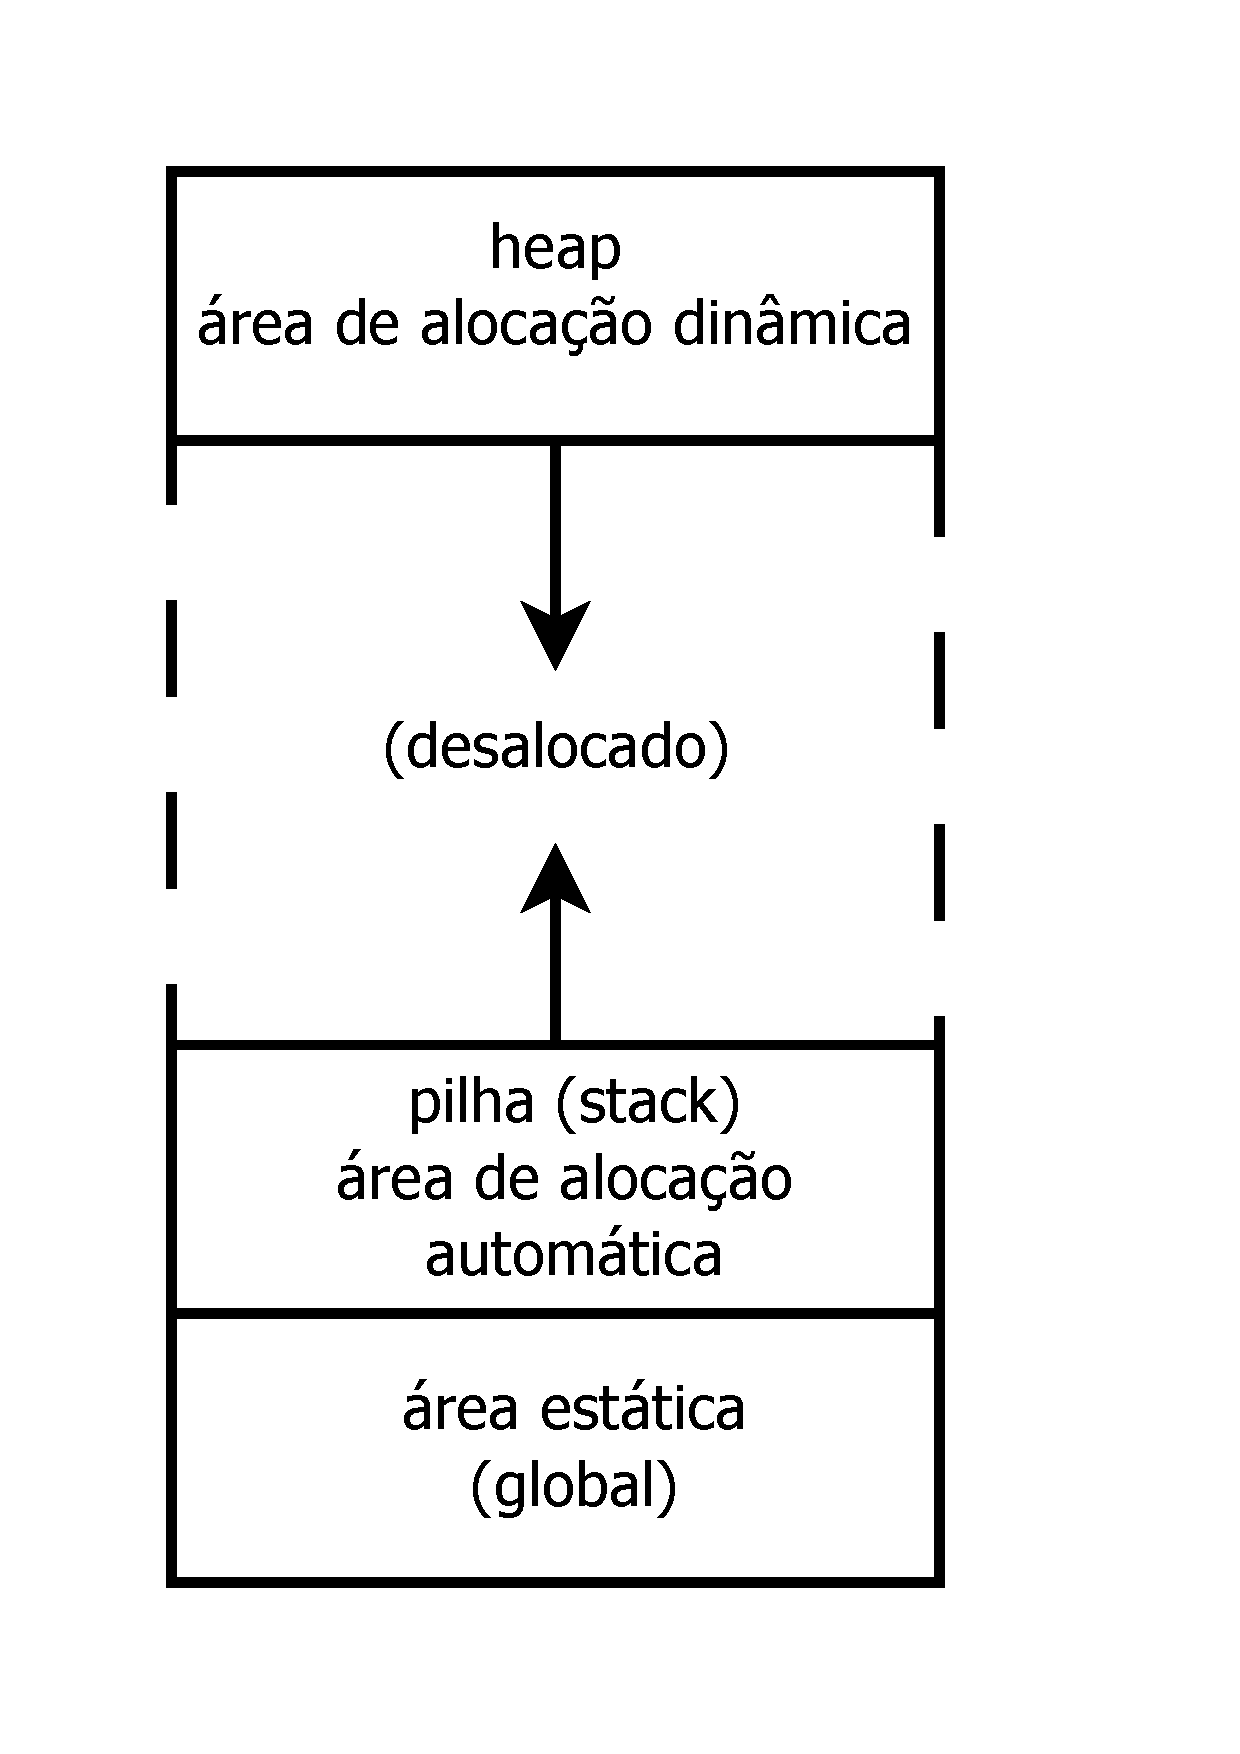
\epsfig{file=figuras/ambiente,width=3cm}		
    \end{block}	

\end{frame}


\section{Escopo}

\begin{frame}[fragile]{Declara\c{c}\~{o}es, blocos e escopo}
\bi
	\item \textbf{Bloco} sequ\^{e}ncia de declara\c{c}\~{o}es seguida de uma sequ\^{e}ncia de instru\c{c}\~{o}es
	\bi
		\item Ling. estruturadas em blocos permitem aninhamento de blocos e redeclara\c{c}\~{a}o de nomes no interior desses blocos.
      	\item \textbf{Declara\c{c}\~{o}es locais} s\~{a}o associadas com algum bloco.
		\item \textbf{Declara\c{c}\~{o}es n\~{a}o locais} s\~{a}o associadas com blocos relacionados.
		\item \textbf{Vari\'{a}veis globais} s\~{a}o tipo particular de vari\'{a}vel n\~{a}o local.
	\ei
\ei

	\begin{block}{Exemplo em C++}
	\begin{lstlisting}[language=c++,numbers=none, basicstyle=\tiny]
      class Shulambs { // bloco de Shulambs
         int i; //declaracao nao local de i para o metodo "f"
         
         void f() {  // bloco aninhado no bloco de Shulambs
            int i;   // declaracao local de i em "f"
         }
      }
	\end{lstlisting}
\end{block}	

\end{frame}

\begin{frame}{Aloca\c{c}\~{a}o, tempo de vida e o ambiente}
	\bi
		\item A mem\'{o}ria para as vari\'{a}veis locais declaradas dentro de uma fun\c{c}\~{a}o n\~{a}o ser\~{a}o alocadas at\'{e} que a fun\c{c}\~{a}o seja chamada.
		\item \textbf{Ativa\c{c}\~{a}o}: chamada a uma fun\c{c}\~{a}o.
		\item \textbf{Registro de ativa\c{c}\~{a}o}: a regi\~{a}o de mem\'{o}ria alocada para aquela chamada de fun\c{c}\~{a}o.
        \item Em uma linguagem baseada em blocos e com escopo l\'{e}xico, o mesmo nome de vari\'{a}vel pode estar associado a diferentes localiza\c{c}\~{o}es (objetos), mas apenas um destes objetos pode ser acessado de cada vez.
	\ei
\end{frame}


\begin{frame}{Escopo}
	\bi
		\item \textbf{Escopo}: trecho do programa em que uma declara\c{c}\~{a}o tem efeito (visibilidade)
		\bi
			\item \textbf{Vari\'{a}vel local}: escopo \'{e} o bloco em que a vari\'{a}vel foi alocada.
			\item \textbf{Vari\'{a}vel global}: escopo \'{e} todo o programa.
		\ei
		\item \textbf{Escopo l\'{e}xico}: em linguagens baseadas em blocos, o escopo \'{e} limitado ao bloco na qual a declara\c{c}\~{a}o aparece (e outros blocos internos a ele)
		\item \textbf{Regra da ``Declara\c{c}\~{a}o antes do uso''}: em linguagens como o C, o escopo de uma declara\c{c}\~{a}o se inicia no ponto da declara\c{c}\~{a}o at\'{e} o final do bloco em que a declara\c{c}\~{a}o est\'{a} localizada
	\ei
\end{frame}



\begin{frame}[fragile]{Escopo de bloco}
	
		\begin{block}{Exemplo em Pascal}
		\centering
    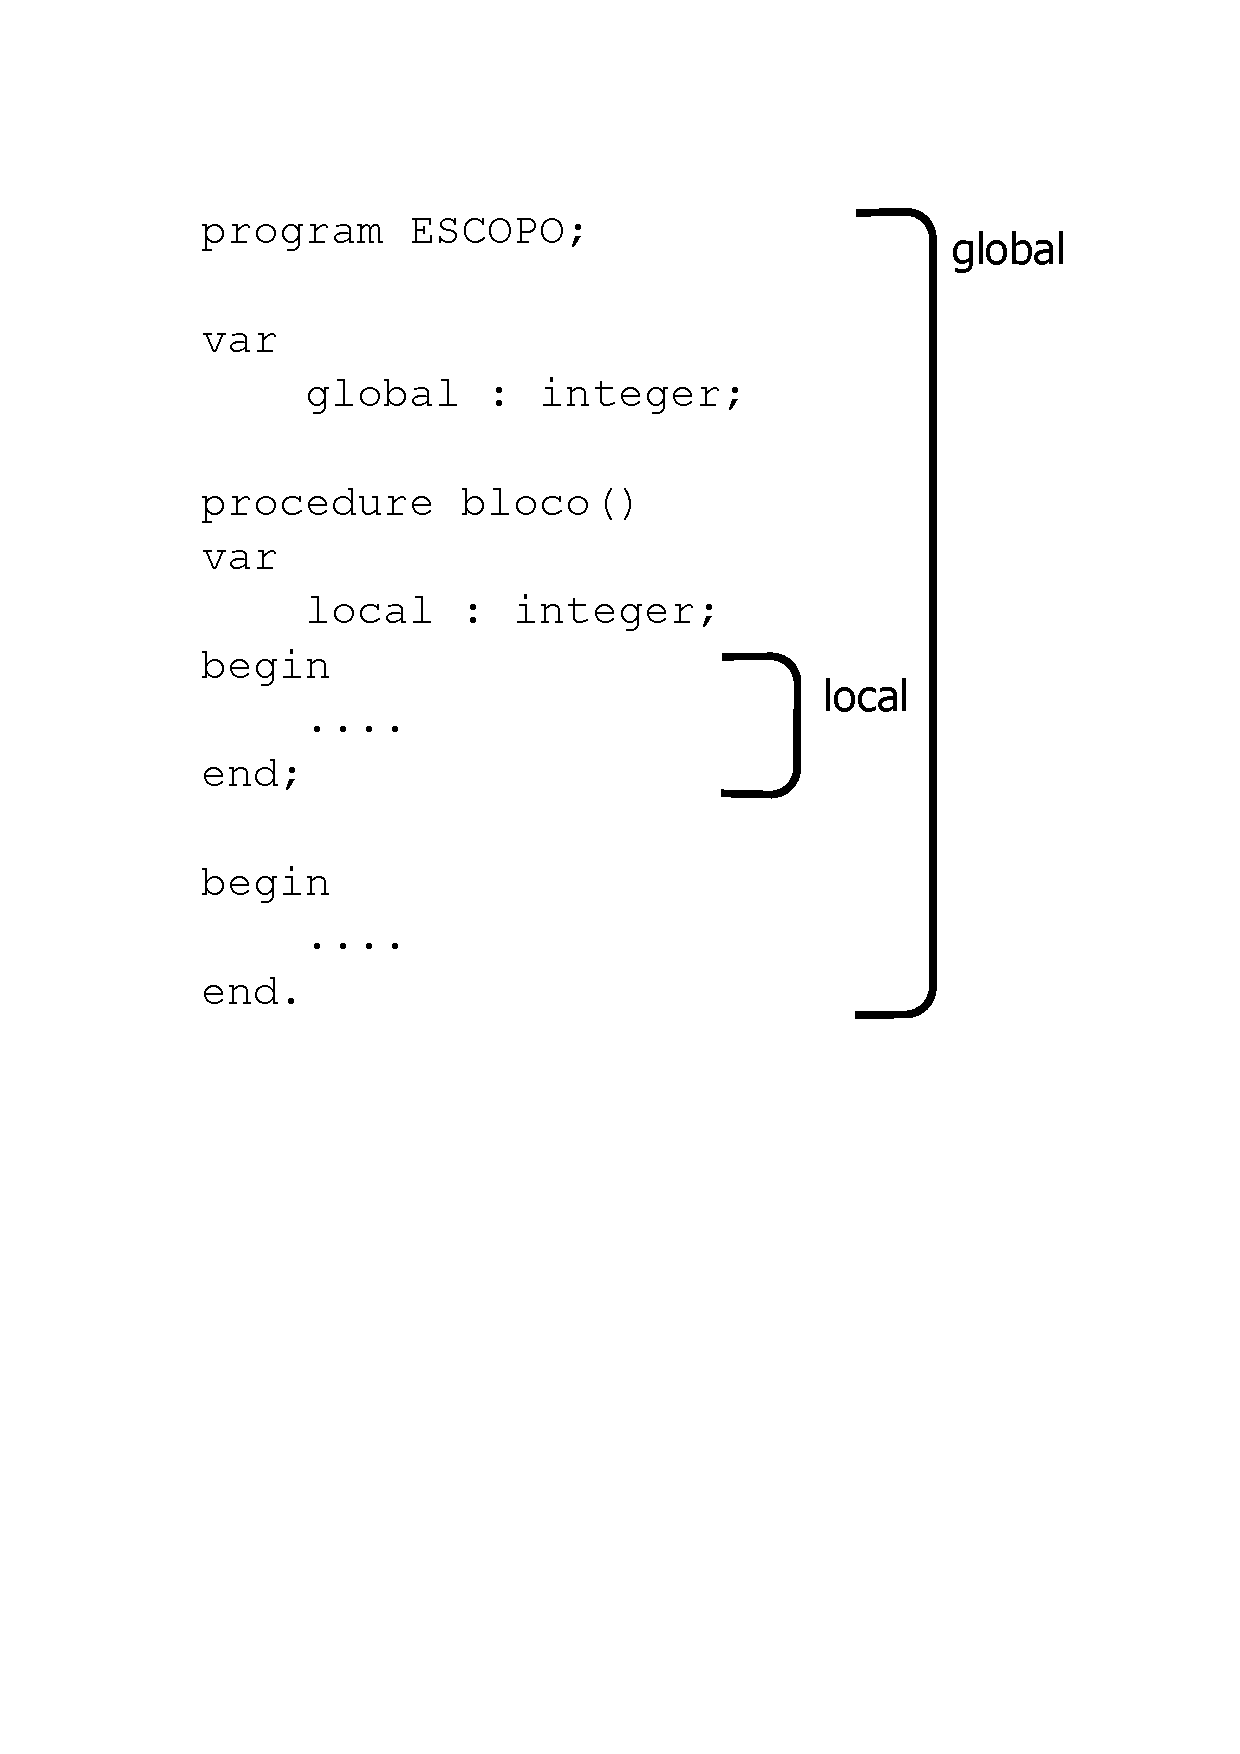
\epsfig{file=figuras/escopoBlocosPascal,width=5.8cm}		
    \end{block}	

\end{frame}



\begin{frame}[fragile]{Regra da ``Declara\c{c}\~{a}o antes do uso''}
	
		\begin{block}{Exemplo em C}
		\centering
    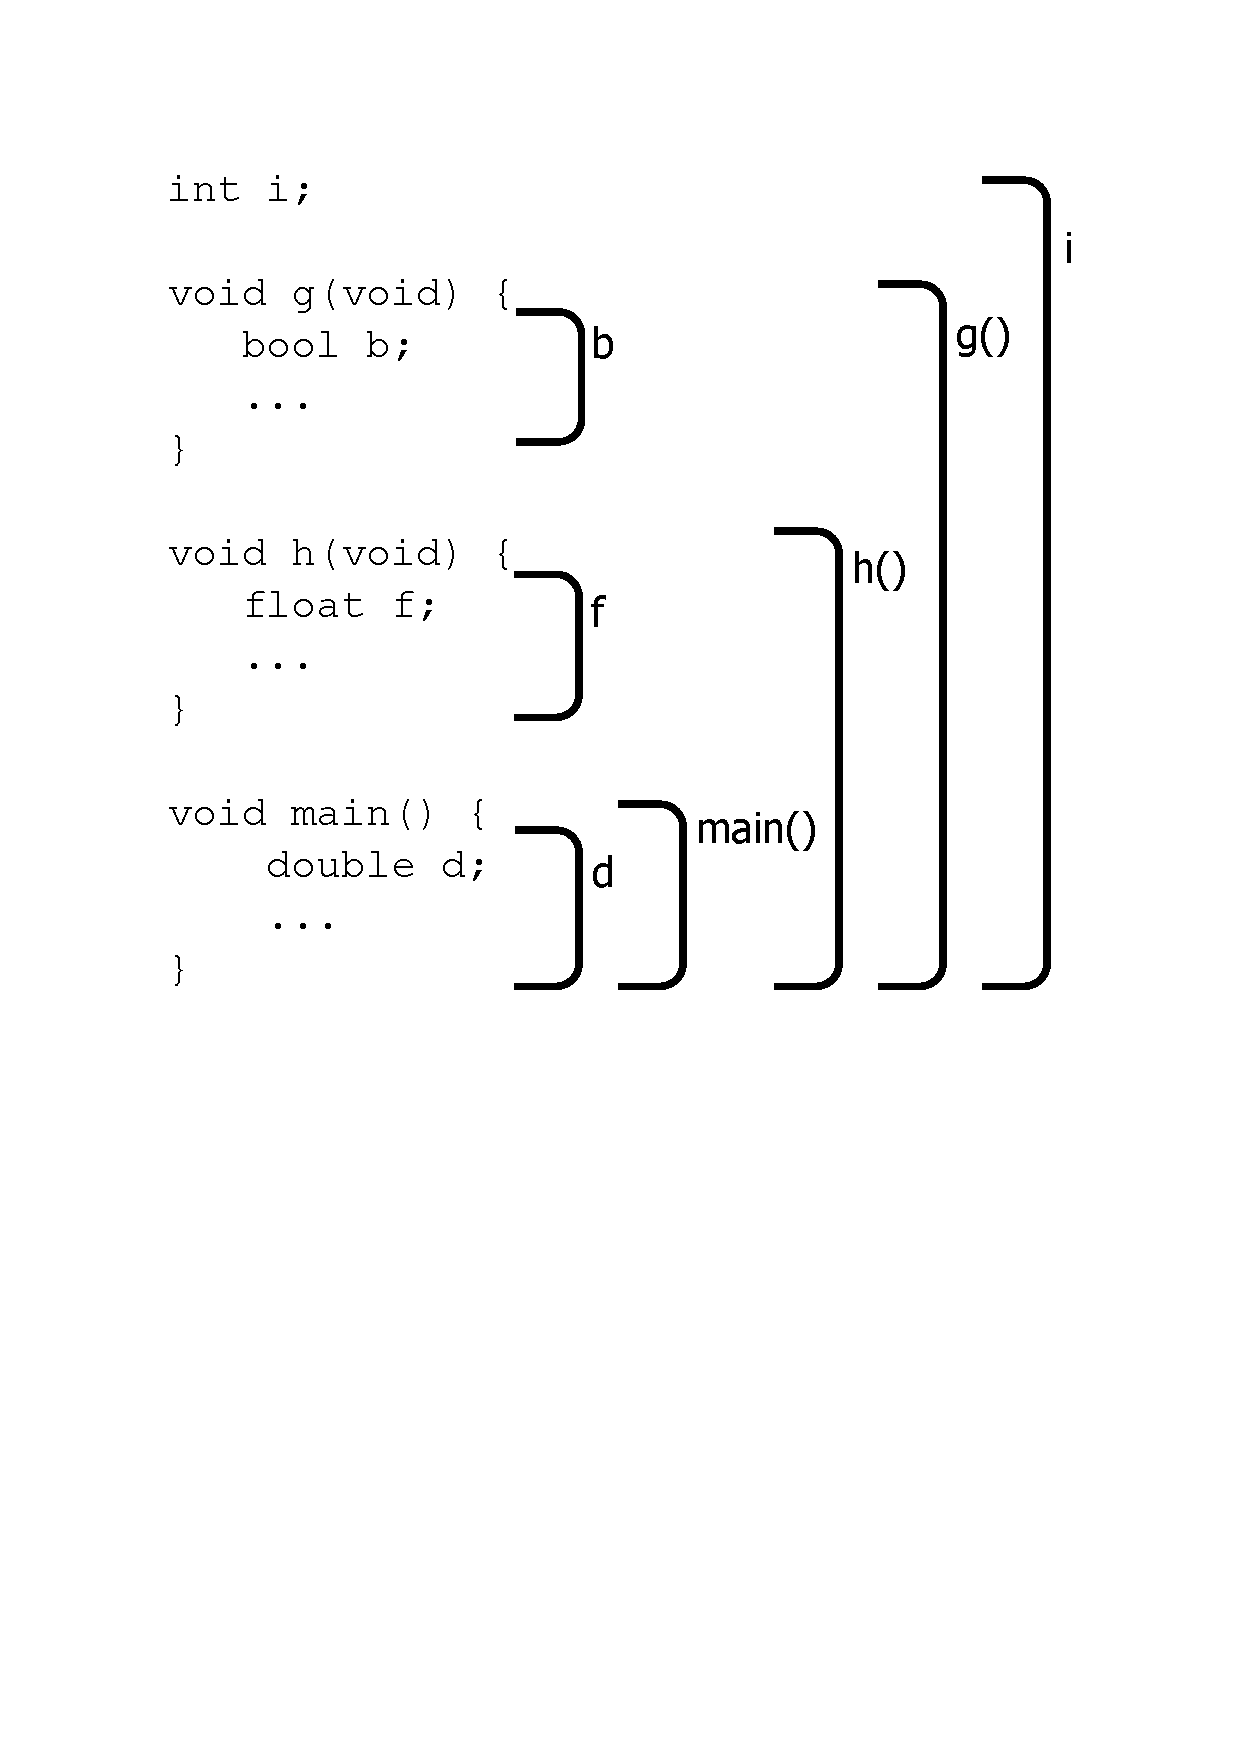
\epsfig{file=figuras/escopoUsoC,width=5.8cm}		
    \end{block}	

\end{frame}


\begin{frame}[fragile]{Tipos de escopo}

   \bi 
   \item Dado um identificador, a que ele est\'{a} associado? Pode ser:
      \bi 
      \item  \emph{Binding} est\'{a}tico (escopo est\'{a}tico ou escopo l\'{e}xico)
      \item  \emph{Binding} din\^{a}mico (escopo din\^{a}mico)
      \ei
	\ei
	
 \begin{block}{Exemplo em C}
 \tiny
	\begin{lstlisting}[language=C,numbers=left]
const int s = 2;
int scale(int x) { 
   return x * s; // a qual declaracao s esta associado ?
} 
int triplica(int x) {
  const int s = 3;
  return scale(x);
}
int main ()  { 
  cout << scale(10) << " e " << triplica(10); 
}
\end{lstlisting}
\end{block}	

\end{frame}


\subsection{Escopo est\'{a}tico}

\begin{frame}{Escopo est\'{a}tico}

   \bi 
   \item Identificador \'{e} associado à declara\c{c}\~{a}o realizada no bloco mais pr\'{o}ximo do ponto de uso do identificador
      \bi 
      \item Blocos s\~{a}o pesquisados ``de dentro para fora''
      \item  \emph{Binding} \'{e} determinado em tempo de compila\c{c}\~{a}o
      \ei
   \item Assim, exemplo anterior ir\'{a} imprimir: 20 e 20
   \item Usado pela grande maioria das linguagens: Algol, Pascal, C, C++, Ada, Java etc
   \item Vantagem:
      \bi 
      \item  Programas mais leg\'{\i}veis e de mais f\'{a}cil entendimento
      \ei
   \ei
\end{frame}

\subsection{Escopo din\^{a}mico}

\begin{frame}{Escopo din\^{a}mico}

   \bi 
   \item Identificador \'{e} associado à declara\c{c}\~{a}o mais pr\'{o}xima na pilha de chamada de subprogramas
      \bi 
      \item  \emph{Binding} \'{e} determinado em tempo de execu\c{c}\~{a}o
      \ei
   \item Assim, exemplo anterior ir\'{a} imprimir: 20 e 30
   \item Usado por linguagens como: LISP (primeiras vers\~{o}es), APL, SNOBOL, Smalltalk, etc
      \bi 
      \item Em geral, linguagens com verifica\c{c}\~{a}o din\^{a}mica de tipos
      \ei
   \item Desvantagens:
      \bi 
      \item Dificulta leitura e entendimento dos programas (\emph{binding} varia com a sequ\^{e}ncia de chamadas de fun\c{c}\~{o}es)
      \item Execu\c{c}\~{a}o mais lenta
      \ei
   \ei
\end{frame}







\begin{frame}[fragile]{Tempo de Vida e Escopo}
	
		\begin{block}{Exemplo em Pascal}
		\centering
    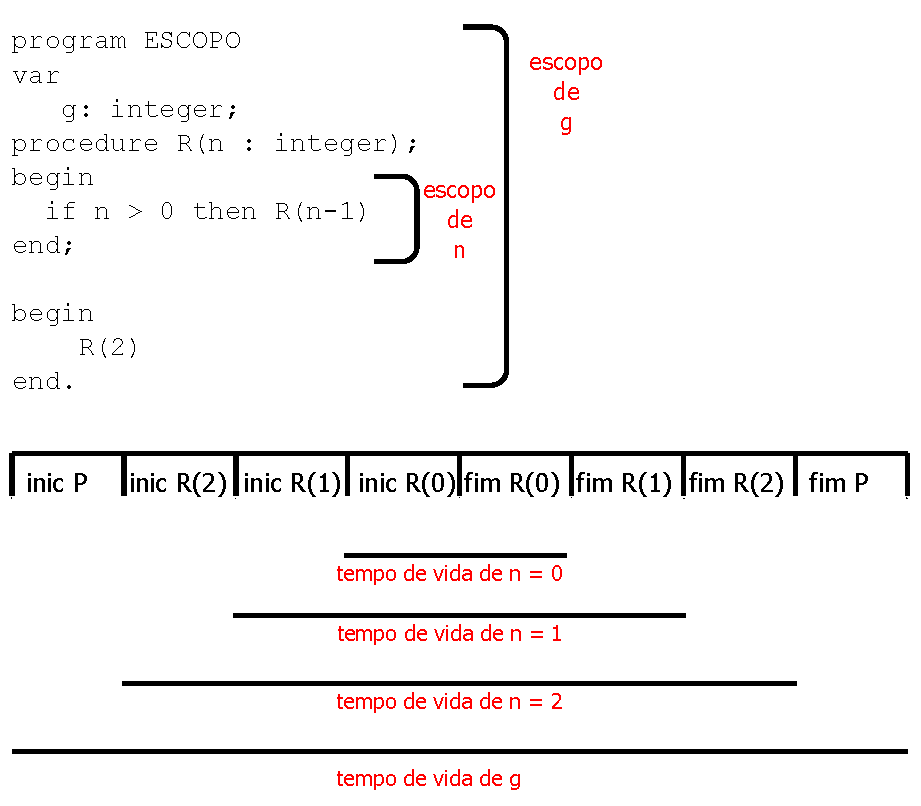
\epsfig{file=figuras/tempoDeVida,width=5.8cm}		
    \end{block}	

\end{frame}

\begin{frame}[fragile]{Vari\'{a}veis est\'{a}ticas}
	\bi
		\item Vari\'{a}vel com escopo local e tempo de vida global
	\ei
	
	\begin{block}{Exemplo em C++}
	\begin{lstlisting}[language=c++,numbers=none,basicstyle=\tiny]
   int a = 1;
  
   void f() {
      int b = 1;         // inicializado a cada chamada de f 
      static int c = a;  // inicializado somente uma vez

      cout << "a = " << a++ << "b = " << b++;
      cout << "c = " << c++ << endl;
      c = c + 2
   }

   int main() {
      while (a < 4)  f();
   }
   \end{lstlisting}
   \end{block}	
\end{frame}

\begin{frame}[fragile]{Alias}

   \bi 
   \item \textbf{Alias} ocorre quando o mesmo objeto \'{e} associado a dois nomes diferentes ao mesmo tempo
   \item Pode surgir durante a chamada de uma fun\c{c}\~{a}o ou procedimento atrav\'{e}s do uso de vari\'{a}veis ponteiro ou refer\^{e}ncia
   \ei

	\begin{block}{Exemplo em C}
	\begin{lstlisting}[language=c,numbers=none, basicstyle=\tiny]
   int *a, *b;
   a = (int *) malloc(sizeof(int));
   *a = 10;
   
   b = a;               // a e b sao alias
   *b = 20;
	
   printf("\%d\n", *a); // ira imprimir 20
   \end{lstlisting}
   \end{block}	
\end{frame}

\begin{frame}{Alias}

   \bi 
   \item Alias pode causar efeitos colaterais indesej\'{a}veis
   \item \textbf{Efeito colateral} \'{e} qualquer mudan\c{c}a no valor de uma vari\'{a}vel que persiste ap\'{o}s a execu\c{c}\~{a}o de uma instru\c{c}\~{a}o (altera o estado global do sistema)
   \item Atribui\c{c}\~{o}es a partir de alias s\~{a}o potencialmente danosas por serem dif\'{\i}ceis de controlar
		\bi
		\item N\~{a}o podem ser determinadas diretamente a partir do c\'{o}digo fonte
		\item n\~{a}o se sabe claramente para onde o ponteiro est\'{a} apontando em um determinado momento.
		\ei
   \ei

\end{frame}


\begin{frame}[fragile]{Refer\^{e}ncia \textit{Dangling}}

   \bi 
   \item Ponteiro que aponta para uma \'{a}rea de mem\'{o}ria que foi liberada
      \bi 
      \item Pode surgir quando o endere\c{c}o de uma vari\'{a}vel local \'{e} atribu\'{\i}do a uma vari\'{a}vel com tempo de vida mais longo
			\ei
   \ei

	\begin{block}{Exemplo em C++}
	\begin{lstlisting}[language=c++,numbers=none,basicstyle=\tiny]
   int *r;

   int f() {
      int v;
      r= &v;
   }
   int main() {
      f();  	
      *r = 1; // r e uma referencia dangling
   }
   \end{lstlisting}
   \end{block}	
\end{frame}


\begin{frame}[fragile]{Lixo}

   \bi 
   \item \textbf{Lixo} \'{e} a mem\'{o}ria que foi alocada no ambiente mas se torna inacess\'{\i}vel ao programa
      \bi 
      \item Pode surgir quando um programador se esquece de desalocar uma vari\'{a}vel din\^{a}mica antes de alterar o estado do ponteiro que referencia esta regi\~{a}o de mem\'{o}ria
			\ei
   \ei

	\begin{block}{Exemplo em C de vazamento de mem\'{o}ria}
	\begin{lstlisting}[language=c++,numbers=none,basicstyle=\tiny]
   int *i;

   i = (int *) malloc(sizeof(int));
   i = 0;
   \end{lstlisting}
   \end{block}	

   \bi 
   \item Programa produz lixo, tamb\'{e}m chamado de vazamento de mem\'{o}ria (\textit{memory leak}) e pode esgotar a mem\'{o}ria do sistema
   \ei
\end{frame}

\begin{frame}{Coletores de lixo}

   \bi 
   \item \textbf{Coletor de lixo} \'{e} um processo que automaticamente elimina o lixo, liberando a mem\'{o}ria que n\~{a}o \'{e} mais utilizada
   \item Coletores de lixo eliminam o vazamento de mem\'{o}ria
   \item Coletores de lixo eliminam refer\^{e}ncias \textit{dangling}
      \bi 
      \item eliminam a necessidade de se desalocar mem\'{o}ria explicitamente
			\ei
   \item Por exemplo: Java
      \bi 
      \item n\~{a}o possui ponteiros expl\'{\i}citos (apenas sem\^{a}ntica de refer\^{e}ncia)
			\item n\~{a}o possui operadores de desaloca\c{c}\~{a}o de mem\'{o}ria (\textit{free} ou \textit{delete})
			\item possui coletor de lixo que faz a gest\~{a}o da desaloca\c{c}\~{a}o de mem\'{o}ria automaticamente
			\ei
   \ei
\end{frame}



\end{document}
